\section {Bond Spectra}

Knowing the orientational behavior of malonic acid helps us to establish a model for how the molecule behaves on an aqueous surface. To link this computationally derived model to our group's experimental work, we turn to the computed spectra of one of the functional moieties of the acid molecules. The bondlengths of the carbonyl C=O bonds were calculated for each simulation at each timestep (similar to the results presented earlier in Figure \ref{fig:bondlength-trajectory}) to generate a time-dependent function, $f(t)$. A calculation was then performed on the time function generate the power spectrum of the bond lengths, hereafter referred to as a ``bond spectrum''. While not fully encapsulating the response of dipole transition moments or recreating IR or SFG spectra, the frequencies captured in a bond spectrum are representational of the local mode frequencies expected from experimental spectroscopic studies, and are directly comparable.

Figure \ref{fig:bond-spectra} shows the C=O carbonyl bond spectrum averaged from all the simulations (top, black spectrum). The two colored spectra in Figure \ref{fig:bond-spectra} show the contributions of the intramolecularly H-bonded and internally unbonded malonic acids, in the bottom and middle spectra, respectively. The coloration of the bottom two plots matches that of Figure \ref{fig:bondlength-distribution}, where the spectral contribution of the carbonyl taking part in the internal H-bond is colored maroon, and the other carbonyl bond response is colored yellow. The color-coded graphic of the molecule for both internal bonding conformations has been reproduced for reference. For the internally unbonded malonic acids, the coloring is more arbitrarily assigned because of the interchangeability of the two bonds.

\begin{figure}[h!]
	\begin{center}
		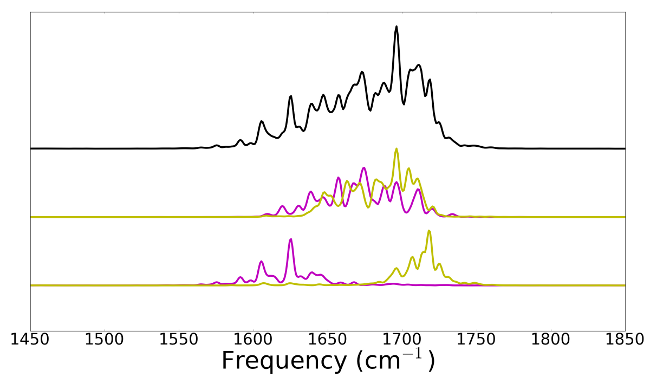
\includegraphics[scale=1.0]{images/bond-spectra/CarbonylBondSpectra.png}
		\caption{}
		\label{fig:bond-spectra}
	\end{center}
\end{figure}



The top spectrum of Figure \ref{fig:bond-spectra} spans approximately 130\cm, with a maximum located towards the upper frequencies near 1700\cm. The width of the spectrum suggests a large distribution of solvation environments in which the carbonyl bonds are interacting with surface waters. In our previous SFG spectroscopic experiments, the response of surface malonic acid molecules was determined to lie within the same spectral range, with peaks centered at ???\cm and ???\cm. The experimental results are very well reproduced in these bond spectra calculations, increasing confidence in the computational method employed for the simulations, and also the consequent picture developed for the orientation and other behaviors of the acid molecules.

To further emphasize the differences between the internally H-bonded and unbonded configurations of malonic acid, the bottom two spectra of Figure \ref{fig:bond-spectra} show the contributions of each set of simulations. The internally unbonded acids have the two ends of the molecule acting more independently than with the internal bond. The two carbonyls can thus both experience a full range of solvation environments. The spectral response of these two carbonyls are expected to be similar, or overlapped in frequencies. As shown in the middle spectrum of Figure \ref{fig:bond-spectra}, the two carbonyl spectra are mostly overlapped, and form the central contributions to the overall spectrum from the collection of all simulation datasets (top of Figure \ref{fig:bond-spectra}). Looking to the bottom spectrum in Figure \ref{fig:bond-spectra}, there is a dramatic splitting of the two carbonyl peaks. The C=O bond involved in the intramolecular H-bond is red-shifted, and the other carbonyl is blue-shifted compared to the internally unbonded spectra. This shift in frequencies shows the strong effect of an internal H-bond on both the bonded carbonyl, and the outer uninvolved carbonyl bond.

In this study, the statistical distribution of the two internal bonding conformations could not be established because of the limited data collected and computational resources used. Thus, the intensities of the spectra can not be directly compared to experimental results, but the frequencies themselves are representational of those for carbonyl bonds. Future studies employing more statistically complete data sets will likely further establish the spectral response of these surface-hydrated malonic acids. Furthermore, it will be possible to establish whether the intramolecularly H-bonded conformation is a statistically relevant species at aqueous surfaces. However, it is possible to conclude that the highest and lower frequency carbonyl responses are contributed by malonic acids with specific geometric conformations (e.g. internal bonding), or some other form of solvation that constrains the motions and interactions of the acid.
